\chapter{EvoOracle: LLMs for Oracles}
\label{cha:evoOracles}
\vspace{0.4 cm}

In this chapter, we introduce EvoOracle, our innovative tool designed for efficient oracle generation using Large Language Models (LLMs). Figure 4.1 provides an insightful overview of EvoOracle's key components and workflow. To initiate the process, we acquire a dataset of Java open-source projects sourced from GitHub. Employing automated test case generation tools such as EvoSuite and Randoop, we systematically create Automated JUnit Test Cases for each project, laying the foundation for EvoOracle's subsequent operations. The tool begins by extracting metadata linked to the identified classes and methods within each project. Subsequently, it mines test cases and establishes mappings with corresponding focal methods extracted from the earlier project analysis. The SUT (System Under Test) Processor component plays a pivotal role in this phase, removing assertions from the test cases and substituting them with placeholders. Following this, the Prompt Processor component takes these test cases, now equipped with placeholders and focal methods, and formulates context for LLM prompting. The LLM Query Processor component utilizes this context to prompt the LLMs, passing the generated responses to the LLM Response Handler component. This handler, in turn, readies the test cases for execution. Finally, the Test Executor compiles and executes the newly generated tests, completing the comprehensive cycle of EvoOracle's oracle generation process.

\begin{figure}[H]
\centering
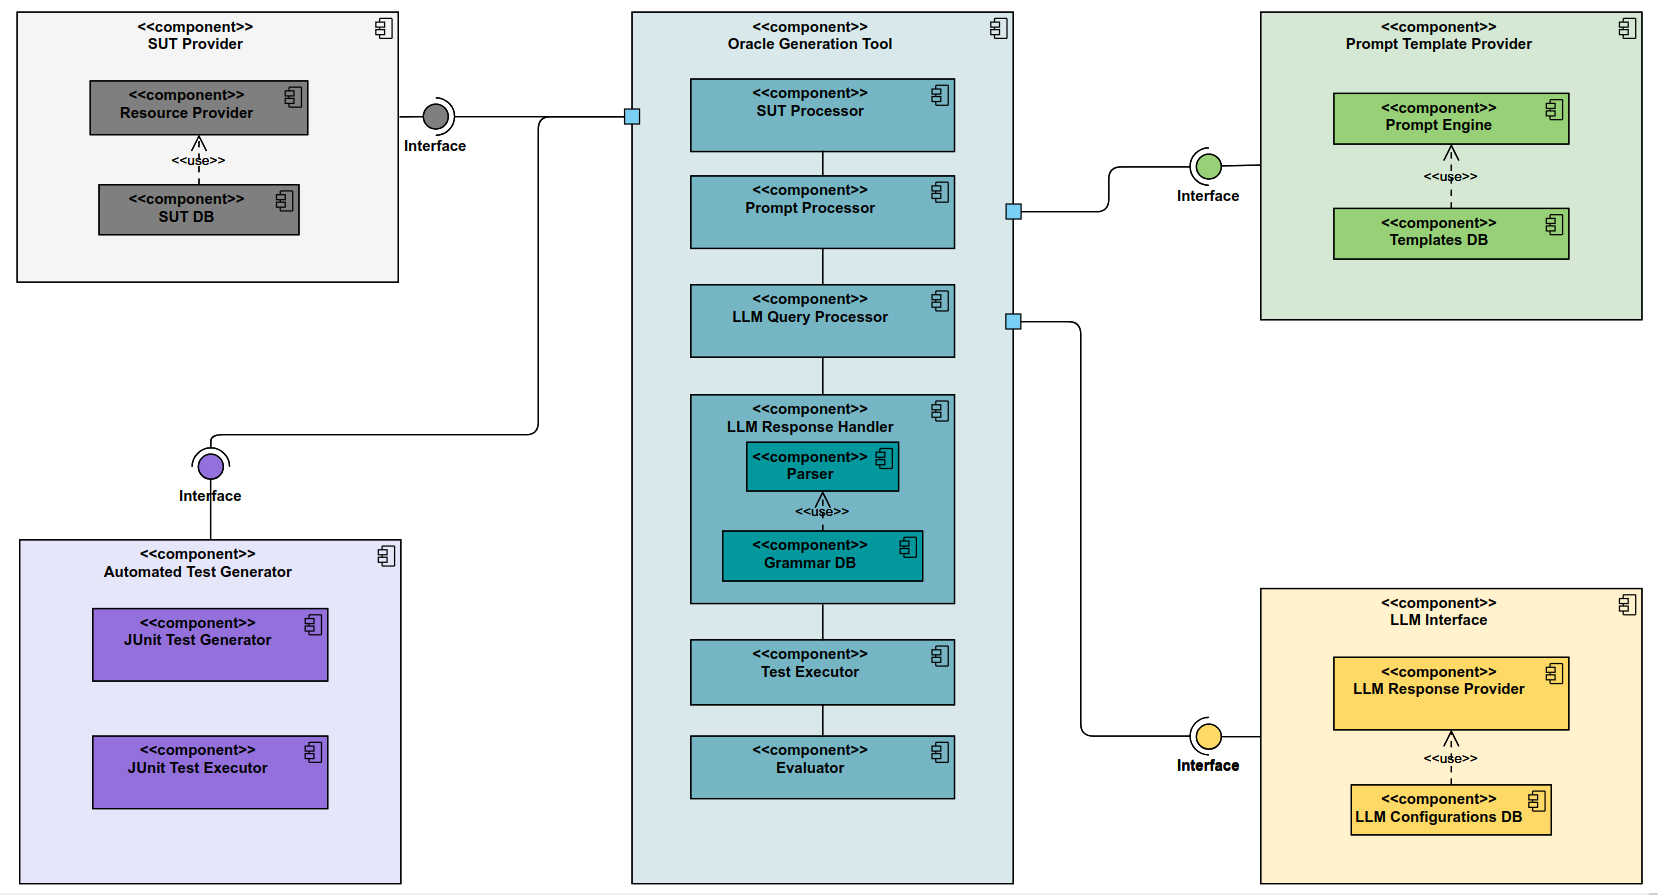
\includegraphics[width=1\textwidth]{images/UML_Component_Diagram_EvoOracle_v2.png}
\caption{Components of our proposed tool: EvoOracle}
\label{fig:component_diagram}
\end{figure}

In the following sub-chapters, we will delve into the intricacies of each step, providing detailed descriptions and insights into the nuances of EvoOracle's comprehensive process.

